\documentclass[12pt,letterpaper]{article}
\usepackage{preamble}
\usepackage[brazil]{babel}
\usepackage[utf8]{inputenc}
\usepackage{enumitem}

%%%%%%%%%%%%%%%%%%%%%%%%%%%%%%%%%%%%%%%%%%
%%%% Edit These for yourself
%%%%%%%%%%%%%%%%%%%%%%%%%%%%%%%%%%%%%%%%%%
\newcommand\course{IA753}
\newcommand\hwnumber{1}
\newcommand\userID{Heitor S. Fernandes}

\begin{document}
\centerline{\textbf{\Large Trabalho Computacional \hwnumber}}

\section*{Questão 1. Análise espectral do ECG}
\begin{enumerate}[label=(\alph*)]  %,leftmargin=!,labelindent=5pt]
    \item Enter your equations and make them left-aligned
        \begin{flalign}
            f(x) &= x^2\\
            g(x) &= \frac{1}{x}\\
            F(x) &= \int^a_b \frac{1}{3}x^3
        \end{flalign}
        
    \item (FFT: mostre o espectro. Qual a resolução espectral?)
    
    \item (Fontes de interferência.) O espectro possui componentes próximas a 50Hz, possivelmente devido à interferência da rede elétrica do local. São observadas, também, componentes em baixas frequências que podem estar relacionadas à respiração ou outros movimentos do indivíduo durante a aquisição do sinal.
        
    \item Adding figures is easy!
        \begin{figure}[H]
            \centering
            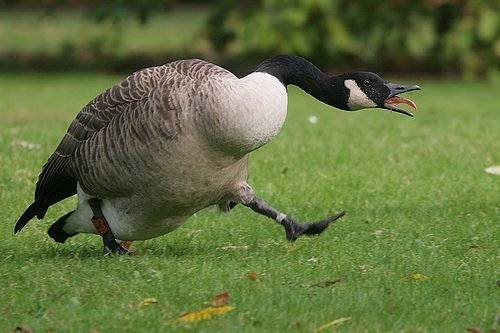
\includegraphics[width=15cm]{images/figure.png}
            \caption{A goose.}
            \label{fig:1}
        \end{figure}
        
    \item To add Matlab code, upload your file and include it here:
        \lstinputlisting[caption={My Matlab script!}]{matlab_files/matlab.m}
        \newpage
    
    \item A console output:
        
        \begin{Verbatim}[frame=single]
Use a Verbatim section to show console output.
All tabs and spaces are shown exactly the way you enter 
them with monospaced font!
        \end{Verbatim}
\end{enumerate}

\newpage
\section*{Question 2}
\setcounter{equation}{0}
\begin{enumerate}[leftmargin=!,labelindent=5pt]
    \item Equations from parts 1 and 2
        \begin{enumerate}
            \item Write the equation of the surface in the form $z = f(x, y)$.
            \begin{flalign}
                f(x)=(x+a)(x+b)\\
                L' = {L}{\sqrt{1-\frac{v^2}{c^2}}} \\
                \lim_{x\to 0}{\frac{e^x-1}{2x}}\\
                \overset{\left[\frac{0}{0}\right]}{\underset{\mathrm{H}}{=}}\\
                \lim_{x\to 0}{\frac{e^x}{2}}={\frac{1}{2}}
            \end{flalign}
        
        \item Make inline math with dollar dollar y'all $woo$! Also centered equations. Tell LaTeX where you want to align equations with \&.
            \begin{align*}
                f(x) &= x^2 \\
                g(x) &= \frac{1}{x} \\
                F(x) &= \int^a_b \frac{1}{3}x^3
            \end{align*}
        \end{enumerate}
    \newpage
    
    \item Plots for Part 3
        \begin{enumerate}
            \item Good times.
                \begin{figure}[H]
                    \centering
                    
\includegraphics[width=15cm]{images/figure3.jpg}
                    \caption{A meme.}
                    \label{fig:3}
                \end{figure}
        \end{enumerate}
\end{enumerate}
\end{document}
